%-----------------------------------------------------------------------------%
\chapter{\babLima}
%-----------------------------------------------------------------------------%


%-----------------------------------------------------------------------------%
\section{Implementasi}
\label{sec:implementation}
%-----------------------------------------------------------------------------%
Algoritma yang disusun pada Bab \ref{sec:design} diimplementasikan dalam bahasa pemrograman. Hasil implementasi kemudian dikombinasikan dengan aplikasi dan \textit{library} pihak ketiga untuk membentuk sebuah \textit{prototype}.


%-----------------------------------------------------------------------------%
\subsection{\textit{Message Broker}}
%-----------------------------------------------------------------------------%
Pada \textit{prototype} yang disusun, \textit{message broker} diimplementasikan dengan menggunakan Redis. Redis merupakan \textit{in-memory data structure store} yang dapat digunakan sebagai \textit{database}, \textit{cache}, dan \textit{message broker} \citep{redis_introduction_2017}. Redis mempunyai \textit{feature} Redis Cluster, sehingga dapat dengan mudah disusun menjadi \textit{distributed system}. Selain itu, Redis Client tersedia dalam hampir semua bahasa pemrograman \textit{mainstream}, sehingga \textit{client} dari \textit{prototype} ini dapat dengan mudah dibuat dalam berbagai versi \citep{redis_clients_2017}.


%-----------------------------------------------------------------------------%
\subsection{\textit{VRP Solver}}
%-----------------------------------------------------------------------------%
VRPSolver yang dirancang dengan mengadopsi algoritma \textit{Cooperative Evolution Algorithms} (CoEAs), diimplementasikan dalam bahasa pemrograman C++. Pemilihan bahasa C++ pada implementasi ini karena permasalahan kombinatorial pada TSP menggunakan resources (prosesor dan memory) yang intensive, sehingga penggunakan C++ dianggap lebih efisien dari bahasa pemrograman lainnya. Source code dari implementasi CoEAs yang digunakan dalam penelitian ini dapat diunduh di \url{https://github.com/soedomoto/coes-mdvrp/tree/jni-coes-mdvrp}. Adapun lingkungan pengembangan Algoritma CoES adalah sebagai berikut:


\begin{itemize}
\item Sistem Operasi		: Elementary OS Loki (Berbasis Ubuntu 16.04)
\item C++ Compiler			: c++ (Ubuntu 5.4.0-6ubuntu1~16.04.4) 5.4.0 20160609
\item Hardware				: Asus TP300L, Quad-Core Intel® Core™ i3-4030U CPU @ 1.90GHz, 3,7 GiB DDRIII, 256GB SSD
\end{itemize}


%-----------------------------------------------------------------------------%
\subsection{\textit{Publisher}}
%-----------------------------------------------------------------------------%
Algoritma yang digunakan untuk publisher, yang meliputi Algoritma \ref{lst:proposed_solver_thread_algorithm} dan Algoritma \ref{lst:proposed_publisher_algorithm}, diimplementasikan dalam bahasa Java. Source code dari implementasi Publisher dapat diunduh di \url{https://github.com/soedomoto/coes-mdvrp/tree/master}. Adapun lingkungan pengembangan Algoritma Publisher adalah sebagai berikut:


\begin{itemize}
\item Sistem Operasi		: Elementary OS Loki (Berbasis Ubuntu 16.04)
\item Java version			: java version "1.8.0\_121"
\item Hardware				: Asus TP300L, Quad-Core Intel® Core™ i3-4030U CPU @ 1.90GHz, 3,7 GiB DDRIII, 256GB SSD
\end{itemize}


%-----------------------------------------------------------------------------%
\section{Pengujian}
\label{sec:testing}
%-----------------------------------------------------------------------------%
Pengujian program dilakukan untuk mengetahui tingkat tercapainya tujuan penelitian ini, yaitu bagaimana membuat rekomendasi lokasi pencacahan pada kondisi data \textit{time windows} tidak tersedia, dan bagaimana menyusun mekanisme \textit{conflict resolution}, agar system tidak merekomendasikan lokasi yang sama pada dua atau lebih pencacah. Ukuran yang akan digunakan dalam pengujian adalah \textit{total cost}, \textit{mean route cost}, dan \textit{route cost mean square error}. Untuk mengukur keakuratan algoritma, maka hasil pengujian akan dibandingkan dengan algoritma MTSP tanpa mekanisme publish/subscribe.


%-----------------------------------------------------------------------------%
\subsection{Lingkungan Pengujian}
%-----------------------------------------------------------------------------%
Pegujian akan dilakukan pada \textit{environment} dengan spesifikasi seperti berikut: 
\begin{itemize}
\item Sistem Operasi		: Elementary OS Loki (Berbasis Ubuntu 16.04)
\item Redis Environment		: Redis 3.2.6, Debian Jessie (Docker version)
\item JRE version			: Java(TM) SE Runtime Environment (build 1.8.0\_121-b13)
\item Database				: H2 Database 1.4.193 (Server mode)
\item Hardware				: Asus TP300L, Quad-Core Intel® Core™ i3-4030U CPU @ 1.90GHz, 3,7 GiB DDRIII, 256GB SSD
\end{itemize}


%-----------------------------------------------------------------------------%
\subsection{\textit{Dataset} dan \textit{Metric}}
%-----------------------------------------------------------------------------%
%-----------------------------------------------------------------------------%
\subsubsection{\textit{Dataset}}
%-----------------------------------------------------------------------------%
Untuk memastikan program dapat bekerja dengan baik, maka program harus diujicobakan dengan berbagai variasi data. Dataset yang paling banyak digunakan dalam pengujian kasus terkait \textit{Vehicle Routing Problem} adalah data Breedam, Cordeau, Solomon, Homberger, dan Russell. Dalam pengujian kali ini akan digunakan dataset Cordeau tipe 2 (Multi-Depot VRP). Dataset Cordeau sendiri tersedia dalam 7 (tujuh) tipe VRP \textit{problem}, antara lain: 

\begin{enumerate}
\item Tipe 0 untuk kasus VRP
\item Tipe 1 untuk kasus Periodic VRP
\item Tipe 2 untuk kasus Multi-Depot VRP
\item Tipe 3 untuk kasus Split Delivery VRP
\item Tipe 4 untuk kasus VRP dengan Time Windows
\item Tipe 5 untuk kasus Periodic VRP dengan Time Windows
\item Tipe 6 untuk kasus Multi-Depot VRP dengan Time Windows
\item Tipe 7 untuk kasus Split Delivery VRP dengan Time Windows
\end{enumerate}


Adapun penjelasan format dari dataset Cordeau tipe 2 adalah sebagai berikut:
\begin{enumerate}
\item Baris pertama berformat \textbf{TYPE M N T}, dimana: \\
M = Jumlah \textit{vehicle} \\
N = Jumlah \textit{customer} \\
T = Jumlah \textit{depot}

\item Baris kedua sampai T baris berikutnya berformat \textbf{D Q}, dimana: \\
D = Durasi maksimum dari setiap rute \\
Q = Kapasitas maksumum dari setiap \textit{vehicle}

\item Baris selanjutnya sampai M baris berikutnya berformat \textbf{i x y d q f a list e l}, dimana: \\
i	= nomer \textit{customer} \\
x	= koordinat x \\
y	= koordinat y \\
d	= durasi pelayanan (\textit{service time}) \\
q	= \textit{demand} \\
f	= frekuensi kunjungan \\
a	= jumlah kombinasi kunjungan \\
list	= list dari semua kombinasi kunjungan \\
e	= jika ada, waktu dimulainya kunjungan \\
l	= jika ada, waktu selesainya kunjungan

\item Baris selanjutnya sampai M baris berikutnya berformat \textbf{i x y}, dimana: \\
i	= nomer \textit{vehicle} \\
x	= koordinat depot x \\
y	= koordinat depot y \\
\end{enumerate}


Selain menggunakan data Cordeau tipe 2, program juga diujicobakan dengan menggunakan data lapangan. Data lapangan yang digunakan meliputi 182 \textit{customers} ($N$) beserta koordinatnya, 15 \textit{vehicle} ($M$) beserta koordinat depot masing-masing \textit{vehicle}. Dari seluruh \textit{customer} dan \textit{vehicle}, dihitung waktu tempuh dari seluruh kombinasi dengan memanfaatkan \textit{Google Direction API}, sebagaimana langkah pada Poin. \ref{ss:distance-duration-matrix}.


%-----------------------------------------------------------------------------%
\subsubsection{\textit{Metric}}
%-----------------------------------------------------------------------------%
Data yang akan digunakan, Cordeau type 2 dan data lapangan, akan diujicobakan dengan menggunakan program usulan, berbasis Pub/Sub dan CoES. Data kemudian diperbandingkan dengan program pembanding yang mengimplementasi algoritma CoES tanpa mekanisme Pub/Sub. Dari kedua program tersebut akan diperoleh output rute untuk masing-masing \textit{vehicle} dengan ilustrasi sebagi berikut:

\begin{itemize}
\item \textit{Vehicle} A = Loc1 -> Loc5 -> Loc15 -> Loc6
\item \textit{Vehicle} B = Loc 6 -> Loc2 -> Loc16 -> Loc3
\item \textit{Vehicle} C = Loc4 -> Loc8 -> Loc14 -> Loc 7
\item \textit{Vehicle} D = Loc9 -> Loc10 -> Loc11 -> Loc12
\end{itemize}


Masing-masing rute kemudian dihitung \textit{total cost}-nya, yang merupakan penjumlahan dari seluruh \textit{service time} pada masing-masing lokasi dan seluruh waktu tempuh dari masing-masing perpindahan. Metric yang akan dijadikan pembanding adalah \textit{mean square error} (MSE) seluruh rute pada masing-masing program dan program pembanding. Program yang lebih baik akan menghasilkan MSE yang lebih kecil. MSE dipilih sebagai \textit{metric} karena merepresentasikan kondisi sebenarnya dilapangan, dimana jika variasi waktu dari seluruh pencacah lebih kecil, maka penyelesaian pencacahan akan lebih merata.


%-----------------------------------------------------------------------------%
\subsection{Skenario dan Hasil Pengujian}
%-----------------------------------------------------------------------------%
Untuk memastikan program dapat bekerja dengan baik, selain menggunakan variasi data, juga akan digunakan berbagai skenario, yaitu:

%-----------------------------------------------------------------------------%
\subsubsection{Pengujian Kondisi Normal}
%-----------------------------------------------------------------------------%
Skenario pengujian kondisi normal dimaksudkan untuk membandingkan program yang dijalankan pada kondisi normal. Pengujian akan dilakukan satu kali untuk masing-masing data set. Pada pengujian ini sebuah program \textit{client} dibuat sebagai simulator.


\begin{figure}[!]
    \centering
    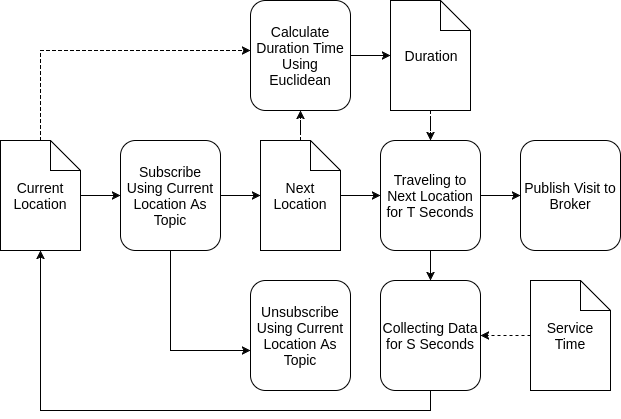
\includegraphics[width=\textwidth]{../../Resources/Images/client-algorithm-nornal-cordeau}
    \caption{\textit{Flowchart} pada \textit{Client Simulator} Kondisi Normal (Cordeau)}
    \label{fig:client-algorithm-nornal-cordeau}
\end{figure}


\begin{figure}[!]
    \centering
    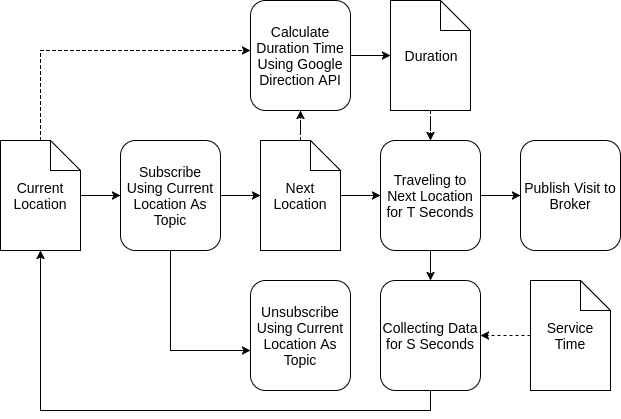
\includegraphics[width=\textwidth]{../../Resources/Images/client-algorithm-nornal-field}
    \caption{\textit{Flowchart} pada \textit{Client Simulator} Kondisi Normal (Lapangan)}
    \label{fig:client-algorithm-nornal-field}
\end{figure}


Langkah-langkah yang diimplementasikan pada program \textit{client}, sebagaimana ilustrasi Gambar \ref{fig:client-algorithm-nornal-cordeau} dan Gambar \ref{fig:client-algorithm-nornal-field}, adalah sebagai berikut:

\begin{enumerate}
\item Buat koneksi dengan \textit{message broker}, 
\item Lakukan \textit{subscription} dengan topik \textit{current location}, 
\item Setelah sebuah \textit{message} diterima, dimana \textit{message} dari \textit{broker} merupakan \textit{next location}, kalkulasi waktu tempuh antara \textit{current location} dengan \textit{next location},
\item Simulasikan perjalanan ke lokasi dengan \textit{sleep},
\item Buat notifikasi terhadap broker atas perubahan \textit{current location}, 
\item Generate \textit{service time}, mengikuti distribusi normal, 
\item Simulasikan pencacahan dengan \textit{sleep}, 
\item Ulangi lagi dari langkah pertama.
\end{enumerate}


Setelah simulasi dilakukan dengan menggunakan dataset Cordeau, diperoleh rute final beserta total durasinya baik untuk algoritma CoES tanpa Pub/Sub maupun untuk algoritma CoES dengan mekanisme Pub/Sub, sebagaimana Tabel \ref{tbl:test_result_normal_cordeau_coes} dan \ref{tbl:test_result_normal_cordeau_pubsub_coes}. Sementara visualisasi rute terdapat pada \autoref{fig:test_result_normal_cordeau_comparison}. Dari hasil pengujian diperoleh perbandingan, sebagaimana Tabel \ref{tbl:test_result_normal_cordeau_comparison}, bahwasannya \textbf{total waktu} yang diperoleh dengan menggunakan CoES lebih kecil, akan tetapi dari sisi \textbf{standar deviasi} dari keseluruhan rute diperoleh hasil metode CoES yang dikombinasikan dengan Pub/Sub menghasilkan angka yang lebih kecil, yang artinya total waktu dari seluruh rute lebih merata.


\begin{longtable}[!]{lp{8cm}r}
	\caption{Hasil Pengujian Kondisi Normal (Cordeau), CoES}
	\label{tbl:test_result_normal_cordeau_coes}\\
	\toprule
		\textit{Vehicle} & Rute & Waktu Total\\ 
	\midrule
	\endfirsthead
	\toprule
		\textit{Vehicle} & Rute & Waktu Total\\ 
	\midrule
	\endhead
	\bottomrule
	\endfoot
		54 & 54-20-3-36-35-29-21 & 135578.58 \\
		51 & 51-42-44-15-37-4-18-17-14-25-13-41-40-19 & 293122.68 \\
		53 & 53-9-50-34-30-10-39-33-45-5-38-11-2-16-49 & 333166.34 \\
		52 & 52-46-12-47-48-24-43-23-7-26-8-31-28-22-1-32-6-27 & 403645.69 \\
\end{longtable}


\begin{longtable}[!]{lp{8cm}r}
	\caption{Hasil Pengujian Kondisi Normal (Cordeau), Pub/Sub CoES}
	\label{tbl:test_result_normal_cordeau_pubsub_coes}\\
	\toprule
		\textit{Vehicle} & Rute & Waktu Total\\ 
	\midrule
	\endfirsthead
	\toprule
		\textit{Vehicle} & Rute & Waktu Total\\ 
	\midrule
	\endhead
	\bottomrule
	\endfoot
		51 & 51-42-19-18-25-14-41-40-13-47-4-12-17-16 & 295641.36 \\
		52 & 52-46-27-24-6-7-23-48-43-8-26-1-31-32 & 310764.56 \\
		53 & 53-49-5-44-37-15-38-11-29-21-34-50-22 & 277819.28 \\
		54 & 54-20-3-28-36-2-35-9-30-10-39-33-45 & 281481.64 \\
\end{longtable}


\begin{longtable}[!]{lrr}
	\caption{Perbandingan Kondisi Normal (Cordeau)}
	\label{tbl:test_result_normal_cordeau_comparison}\\
	\toprule
		\textit{Vehicle} & Rute & Waktu Total\\ 
	\midrule
	\endfirsthead
	\toprule
		\textit{Vehicle} & Rute & Waktu Total\\ 
	\midrule
	\endhead
	\bottomrule
	\endfoot
		Total Waktu & 1165513.28 & 1165706.84\\
		Rata-rata & 291378.32 & 291426.71\\
		Standar Deviasi & 98268.51 & 12997.91\\
\end{longtable}


\begin{figure*}[!]
    \centering
    \begin{subfigure}[t]{0.5\textwidth}
        \centering
		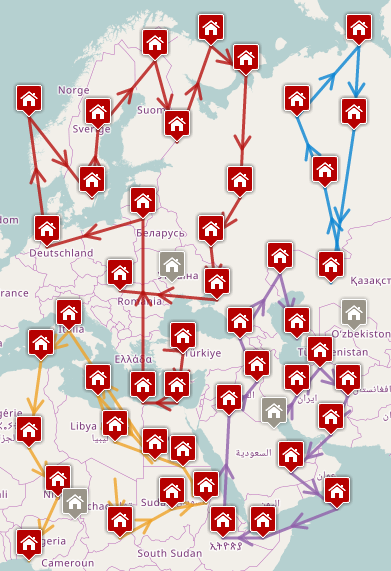
\includegraphics[width=\textwidth]{../../Resources/Images/test_result_normal_cordeau_coes}
		\caption{CoES}
		\label{fig:test_result_normal_cordeau_pubsub_coes}
    \end{subfigure}%
    ~ 
    \begin{subfigure}[t]{0.5\textwidth}
        \centering
		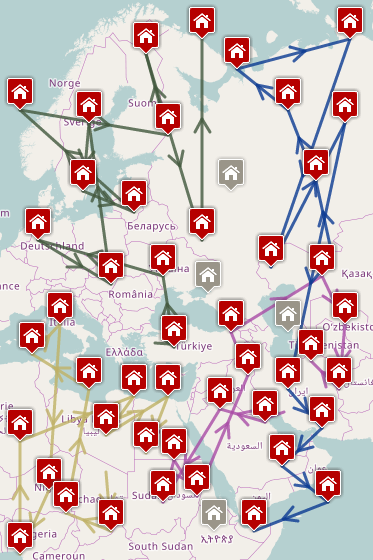
\includegraphics[width=\textwidth]{../../Resources/Images/test_result_normal_cordeau_pubsub_coes}
		\caption{Pub/Sub CoES}
		\label{fig:test_result_normal_cordeau_pubsub_coes}
    \end{subfigure}
    \caption{Perbandingan Rute Kondisi Normal (Cordeau)}
    \label{fig:test_result_normal_cordeau_comparison}
\end{figure*}


Sementara itu, pengujian dengan menggunakan data lapangan, rute yang diperoleh sebagaimana Tabel \ref{tbl:test_result_normal_field_coes} untuk algoritma CoES, dan Tabel \ref{tbl:test_result_normal_field_pubsub_coes} untuk algoritma CoES dengan mekanisme Pub/Sub. Dari hasil pengujian, sebagaimana Tabel \ref{tbl:test_result_normal_field_comparison}, menghasilkan kesimpulan yang tidak jauh berbeda dengan Tabel \ref{tbl:test_result_normal_cordeau_comparison}, dimana algoritma CoES menghasilkan \textbf{waktu total} yang lebih kecil dibandingkan algoritma CoES yang dikombinasikan dengan Pub/Sub, tetapi dari sisi \textbf{standar deviasi} lebih besar.


\begin{longtable}[!]{lp{8cm}r}
	\caption{Hasil Pengujian Kondisi Normal (Lapangan), CoES}
	\label{tbl:test_result_normal_field_coes}\\
	\toprule
		\textit{Vehicle} & Rute & Waktu Total\\ 
	\midrule
	\endfirsthead
	\toprule
		\textit{Vehicle} & Rute & Waktu Total\\ 
	\midrule
	\endhead
	\bottomrule
	\endfoot
		1302021005 & 1302021005-1302021005-1302020010-1302020001-1302020009-1302020011-1302021001 & 143455.33 \\
		1302090004 & 1302090004-1302090008-1302090002-1302090007-1302090005-1302090001-1302090015-1302090009-1302090014-1302090003-1302090018-1302090016-1302090017-1302090013-1302090012-1302090006-1302090004-1302090019-1302090020 & 429950.94 \\
		1302011008 & 1302011008-1302011008-1302011010-1302011001-1302012005-1302011007-1302011009-1302011004-1302011003-1302011002-1302011006-1302011005 & 264181.29 \\
		1302031005 & 1302031005-1302031001-1302031006-1302031008-1302040011-1302031009-1302031010-1302031007-1302030001-1302031002-1302031005 & 246533.56 \\
		1302050007 & 1302050007-1302050007-1302050008-1302050009-1302050010-1302050002-1302050006 & 146835.04 \\
		1302100002 & 1302100002-1302100002-1302100009-1302100008-1302100007-1302100006-1302100001-1302100017-1302100016-1302090011-1302090010-1302100004-1302100015-1302100003-1302100013-1302100012 & 377098.71 \\
		1302030005 & 1302030005-1302030005-1302030014-1302030006-1302030009-1302030004-1302030012-1302030003-1302031004-1302031003-1302030002-1302030010 & 261871.21 \\
		1302012003 & 1302012003-1302012008-1302012003-1302012001-1302012006-1302012002-1302012010-1302012009-1302012004-1302012007 & 218170.80 \\
		1302080006 & 1302080006-1302080006-1302080004-1302080009-1302080003-1302080005-1302080001-1302080008-1302080002-1302080007 & 226083.58 \\
		1302070006 & 1302070006-1302070006-1302070002-1302070011-1302070003-1302070012-1302070005-1302070007-1302070008-1302070009-1302070010-1302070004-1302070001 & 299255.93 \\
		1302060005 & 1302060005-1302060005-1302060009-1302060006-1302060008-1302060002-1302060007-1302060001-1302060003-1302060004 & 215375.02 \\
		1302020006 & 1302020006-1302020006-1302020017-1302020016-1302020015-1302021002-1302021008-1302021003-1302021009-1302021010-1302021004-1302021007-1302021006-1302020005-1302020003 & 347975.49 \\
		1302110003 & 1302110003-1302110019-1302110018-1302110012-1302110023-1302110006-1302110021-1302110008-1302110007-1302110022-1302110009-1302110020-1302110005-1302110004-1302110010-1302100005-1302110001-1302110013-1302110002-1302110014-1302110015-1302110017-1302110016-1302110011-1302110003 & 600827.54 \\
		1302040002 & 1302040002-1302040004-1302040003-1302040015-1302040001-1302040008-1302040009-1302040010-1302040012-1302040014-1302040013-1302040002-1302040016-1302050003-1302050005-1302050004-1302050001-1302040005-1302040006-1302040007 & 445481.39 \\
		1302101005 & 1302101005-1302101005-1302100010-1302101002-1302101003-1302101006-1302101004-1302100011-1302100014-1302101001 & 225893.85 \\
\end{longtable}


\begin{longtable}[!]{lp{8cm}r}
	\caption{Hasil Pengujian Kondisi Normal (Lapangan), Pub/Sub CoES}
	\label{tbl:test_result_normal_field_pubsub_coes}\\
	\toprule
		\textit{Vehicle} & Rute & Waktu Total\\ 
	\midrule
	\endfirsthead
	\toprule
		\textit{Vehicle} & Rute & Waktu Total\\ 
	\midrule
	\endhead
	\bottomrule
	\endfoot
		1302011008 & 1302011008-1302011008-1302011010-1302011001-1302012005-1302011007-1302011009-1302011005-1302011004-1302011006-1302011002-1302110008 & 288136.01 \\
		1302040002 & 1302040002-1302040004-1302040002-1302040003-1302040015-1302040001-1302040008-1302040009-1302040010-1302040016-1302040013-1302040012 & 260428.46 \\
		1302012003 & 1302012003-1302012008-1302012001-1302012006-1302012002-1302012004-1302012010-1302012009-1302020001-1302011003-1302040014-1302110022 & 289894.14 \\
		1302060005 & 1302060005-1302060005-1302060009-1302060006-1302060008-1302060002-1302060007-1302060001-1302060004-1302060003-1302040007-1302040005 & 263996.44 \\
		1302020006 & 1302020006-1302020006-1302020016-1302020017-1302020015-1302021002-1302021006-1302020005-1302020003-1302021007-1302021003-1302021009 & 271963.26 \\
		1302080006 & 1302080006-1302080006-1302080009-1302080005-1302080002-1302080008-1302080007-1302080001-1302080003-1302070008-1302070004-1302100005-1302110014-1302110013-1302110009 & 357607.07 \\
		1302021005 & 1302021005-1302021005-1302021001-1302012003-1302012007-1302020010-1302020011-1302020009-1302021010-1302021004-1302021008-1302110017-1302110002 & 309232.92 \\
		1302100002 & 1302100002-1302100002-1302100003-1302100009-1302100006-1302100008-1302100013-1302101001-1302100012-1302100004-1302100015-1302100016-1302090010-1302090011-1302100001-1302100017 & 382894.06 \\
		1302101005 & 1302101005-1302101005-1302100010-1302100014-1302100011-1302101004-1302101006-1302101003-1302101002-1302100007-1302090005-1302110015-1302110011 & 301312.52 \\
		1302110003 & 1302110003-1302110019-1302110004-1302110018-1302110001-1302110010-1302110020-1302110006-1302110023-1302110012-1302110005-1302110003-1302110016 & 294736.00 \\
		1302090004 & 1302090004-1302090008-1302090001-1302090015-1302090013-1302090012-1302090006-1302090002-1302090007-1302090009-1302090003-1302090018-1302090016-1302090014-1302090017 & 334625.82 \\
		1302030005 & 1302030005-1302030005-1302030014-1302030006-1302030009-1302030012-1302030004-1302030010-1302031004-1302030003-1302030002-1302031003-1302110021-1302110007 & 330329.51 \\
		1302070006 & 1302070006-1302070006-1302070002-1302070011-1302070005-1302080004-1302070003-1302070012-1302070007-1302070001-1302070009-1302070010 & 277740.88 \\
		1302050007 & 1302050007-1302050007-1302050006-1302050004-1302050003-1302050005-1302050009-1302050010-1302050002-1302050008-1302050001-1302090004-1302090020-1302090019 & 323349.34 \\
		1302031005 & 1302031005-1302031001-1302031006-1302031008-1302040011-1302031009-1302031010-1302031002-1302031007-1302030001-1302031005-1302040006 & 273412.25 \\
\end{longtable}


\begin{longtable}[!]{lrr}
	\caption{Komparasi CoES dan Pub/Sub + CoES pada Data Lapangan}
	\label{tbl:test_result_normal_field_comparison}\\
	\toprule
		Ukuran & CoES & CoES + Pub/Sub\\ 
	\midrule
	\endfirsthead
	\toprule
		Ukuran & CoES & CoES + Pub/Sub\\ 
	\midrule
	\endhead
	\bottomrule
	\endfoot
		Total Waktu & 4448989.67 & 4559658.67\\
		Rata-rata & 296599.31 & 303977.24\\
		Standar Deviasi & 119720.84 & 34472.12\\
\end{longtable}


\begin{figure*}[!]
    \centering
    \begin{subfigure}[t]{0.5\textwidth}
        \centering
		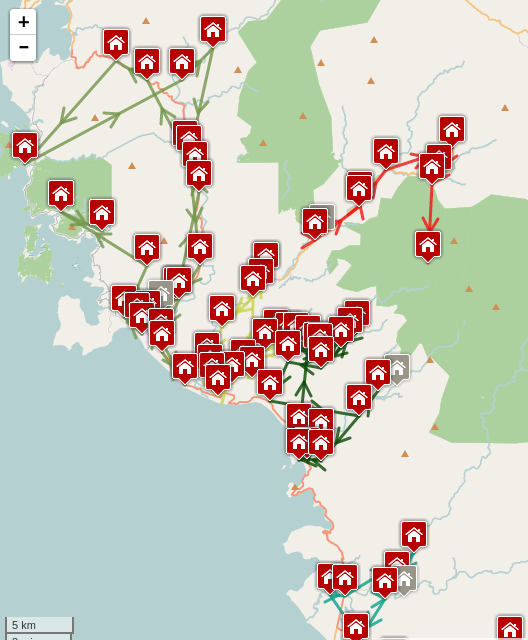
\includegraphics[width=\textwidth]{../../Resources/Images/test_result_normal_field_coes}
		\caption{CoES}
		\label{fig:test_result_normal_field_coes}
    \end{subfigure}%
    ~ 
    \begin{subfigure}[t]{0.5\textwidth}
        \centering
		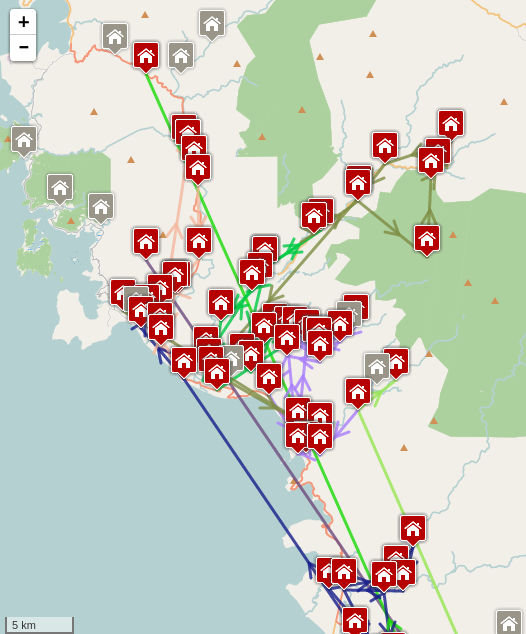
\includegraphics[width=\textwidth]{../../Resources/Images/test_result_normal_field_pubsub_coes}
		\caption{Pub/Sub CoES}
		\label{fig:test_result_normal_field_pubsub_coes}
    \end{subfigure}
    \caption{Perbandingan Rute Kondisi Normal (Cordeau)}
    \label{fig:test_result_normal_field_comparison}
\end{figure*}


%-----------------------------------------------------------------------------%
\subsubsection{Pengujian Kondisi \textit{Unstable Connection}}
%-----------------------------------------------------------------------------%
Skenario pengujian kondisi \textit{unstable connection} dimaksudkan untuk membandingkan program yang dijalankan pada kondisi dimana terjadi \textit{delay} secara random. Pengujian ini digunakan sebagai cerminan kodisi lapangan dimana pada beberapa lokasi tidak terdapat koneksi yang stabil. Pengujian akan dilakukan satu kali untuk data lapangan. Pada pengujian ini sebuah program \textit{client} juga dirancang sebagai simulator.


\begin{figure}[!]
    \centering
    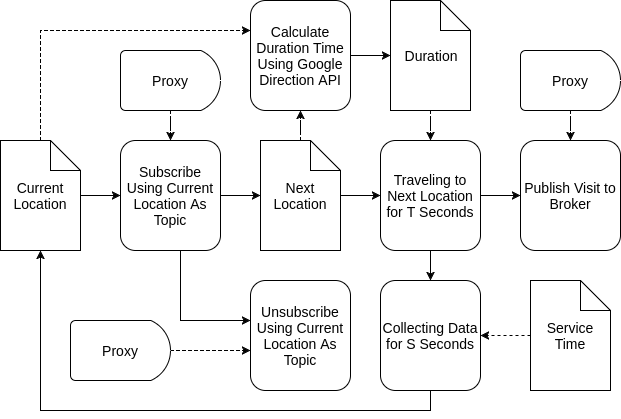
\includegraphics[width=\textwidth]{../../Resources/Images/client-algorithm-unstable-connection-field}
    \caption{\textit{Flowchart} pada \textit{Client Simulator} Kondisi \textit{Unstable Connection}}
    \label{fig:client-algorithm-unstable-connection-field}
\end{figure}


Langkah-langkah yang diimplementasikan pada program \textit{client}, sebagaimana ilustrasi Gambar \ref{fig:client-algorithm-unstable-connection-field}, adalah sebagai berikut:

\begin{enumerate}
\item Buat sebuah \textit{forward proxy server} yang mengimplementasikan \textit{random delay}, dengan destinasi adalah IP dari \textit{message broker}, 
\item Setiap komunikasi dengan \textit{message broker} harus melalui \textit{forward proxy server}, 
\item Buat koneksi dengan \textit{message broker}, 
\item Lakukan \textit{subscription} dengan topik \textit{current location}, 
\item Setelah sebuah \textit{message} diterima, dimana \textit{message} dari \textit{broker} merupakan \textit{next location}, kalkulasi waktu tempuh antara \textit{current location} dengan \textit{next location},
\item Simulasikan perjalanan ke lokasi dengan \textit{sleep},
\item Buat notifikasi terhadap broker atas perubahan \textit{current location}, 
\item Generate \textit{service time}, mengikuti distribusi normal, 
\item Simulasikan pencacahan dengan \textit{sleep}, 
\item Ulangi lagi dari langkah pertama.
\end{enumerate}


%-----------------------------------------------------------------------------%
\subsubsection{Pengujian Kondisi Pencacah Berhenti}
%-----------------------------------------------------------------------------%
Skenario pengujian kondisi normal dimaksudkan untuk membandingkan program yang dijalankan pada kondisi dimana satu atau lebih pencacah berhenti ditengah jalan. Pengujian akan dilakukan satu kali untuk data lapangan. Pada pengujian ini sebuah program \textit{client} dirancang sebagai simulator.


\begin{figure}[!]
    \centering
    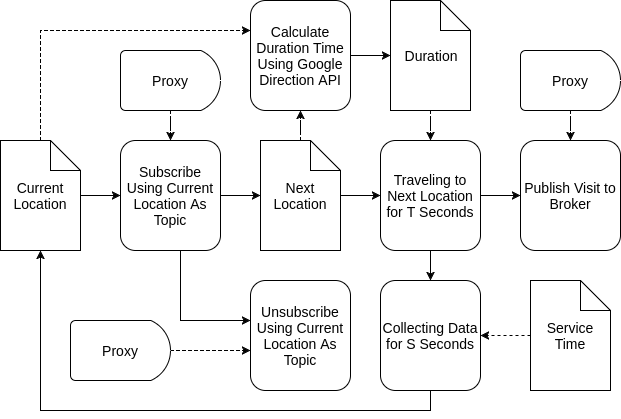
\includegraphics[width=\textwidth]{../../Resources/Images/client-algorithm-enumerator-quit-field}
    \caption{\textit{Flowchart} pada \textit{Client Simulator} Kondisi Pencacah Berhenti}
    \label{fig:client-algorithm-enumerator-quit-field}
\end{figure}


Langkah-langkah yang diimplementasikan pada program \textit{client}, sebagaimana ilustrasi Gambar \ref{fig:client-algorithm-enumerator-quit-field}, adalah sebagai berikut:

\begin{enumerate}
\item Buat koneksi dengan \textit{message broker}, 
\item Lakukan \textit{subscription} dengan topik \textit{current location}, 
\item Setelah sebuah \textit{message} diterima, dimana \textit{message} dari \textit{broker} merupakan \textit{next location}, kalkulasi waktu tempuh antara \textit{current location} dengan \textit{next location},
\item Simulasikan perjalanan ke lokasi dengan \textit{sleep},
\item Buat notifikasi terhadap broker atas perubahan \textit{current location}, 
\item Generate \textit{service time}, mengikuti distribusi normal, 
\item Simulasikan pencacahan dengan \textit{sleep}, 
\item Hentikan beberapa proses, 
\item Ulangi lagi dari langkah pertama.
\end{enumerate}


Pada pengujian ini, disimulasikan bahwasannya pencacah 1302110003 berhenti setelah 150000 detik, 1302101005 setelah 360000 detik, 1302012003 setelah 180000 detik, dan 1302080006 setelah 300000 detik. Tabel \ref{tbl:test_result_enumerator_quit_field_pubsub_coes} menunjukkan hasil simulasi dan waktu total untuk masing-masing pencacah. Ketika rute dari keempat pencacah tersebut dikeluarkan dari penghitungan standar deviasi, maka sebagaimana Tabel \ref{tbl:test_result_enumerator_quit_field} diperoleh .


\begin{longtable}[!]{lp{8cm}r}
	\caption{Hasil Pengujian Kondisi Pencacah Berhenti}
	\label{tbl:test_result_enumerator_quit_field_pubsub_coes}\\
	\toprule
		\textit{Vehicle} & Rute & Waktu Total\\ 
	\midrule
	\endfirsthead
	\toprule
		\textit{Vehicle} & Rute & Waktu Total\\ 
	\midrule
	\endhead
	\bottomrule
	\endfoot
		1302011008 & 1302011008-1302011008-1302011010-1302011001-1302012005-1302011007-1302011009-1302011005-1302011006-1302011002-1302011004-1302011003-1302090007-1302090015-1302110002-1302110013-1302110006 & 407401.10 \\
		1302040002 & 1302040002-1302040002-1302040016-1302040004-1302040005-1302040006-1302040015-1302040007-1302040003-1302040009-1302040013-1302040008-1302090013 & 306233.49 \\
		1302012003 & 1302012003-1302012008-1302012003-1302012001-1302012006-1302012002-1302012004-1302012010 & 169070.15 \\
		1302060005 & 1302060005-1302060005-1302060009-1302060006-1302060008-1302060007-1302060001-1302060004-1302050010-1302050009-1302060003-1302012009-1302100016-1302090010 & 345013.89 \\
		1302020006 & 1302020006-1302020006-1302020016-1302020015-1302021002-1302021006-1302020017-1302031005 & 171648.83 \\
		1302080006 & 1302080006-1302080006-1302080007-1302080008-1302080002-1302080001-1302080004-1302080009-1302070012-1302070003-1302080003-1302080005 & 269836.91 \\
		1302021005 & 1302021005-1302021005-1302021001-1302020011-1302020009-1302020001-1302020010-1302021003-1302021008-1302021010-1302021007-1302021009-1302021004-1302110012 & 335580.21 \\
		1302100002 & 1302100002-1302100002-1302100003-1302100013-1302100009-1302100001-1302100005-1302110023-1302110021-1302110022-1302110008-1302110007-1302110020-1302110018-1302110009-1302110003-1302110010-1302110005 & 428783.15 \\
		1302101005 & 1302101005-1302101005-1302100010-1302101002-1302100014-1302100011-1302101003-1302101001-1302100006-1302100004-1302100012-1302100007-1302100017-1302101004 & 327886.72 \\
		1302110003 & 1302110003-1302110019-1302110004-1302110001-1302110011-1302110017-1302110016 & 147061.67 \\
		1302090004 & 1302090004-1302090008-1302090002-1302090005-1302090004-1302090012-1302090014-1302090020-1302090019-1302090001-1302090017-1302090018-1302090016-1302110014-1302101006-1302090011 & 368625.31 \\
		1302030005 & 1302030005-1302030005-1302030014-1302030006-1302030009-1302030004-1302030012-1302030003-1302031004-1302030010-1302030002-1302031003-1302020005-1302020003-1302100015-1302100008 & 382133.70 \\
		1302070006 & 1302070006-1302070006-1302070002-1302070011-1302070005-1302070008-1302070009-1302070010-1302070007-1302070001-1302070004-1302060002-1302110015 & 299606.48 \\
		1302050007 & 1302050007-1302050007-1302050008-1302050002-1302050006-1302050004-1302050001-1302050003-1302050005-1302040001-1302040012-1302012007-1302090006-1302090009-1302090003 & 369932.48 \\
		1302031005 & 1302031005-1302031001-1302031006-1302031008-1302040011-1302031009-1302031010-1302040010-1302031007-1302030001-1302031002-1302040014 & 278953.18 \\
\end{longtable}


\begin{longtable}[!]{lrr}
	\caption{Komparasi CoES dan Pub/Sub + CoES pada Data Lapangan}
	\label{tbl:test_result_enumerator_quit_field}\\
	\toprule
		Ukuran & CoES & CoES + Pub/Sub\\ 
	\midrule
	\endfirsthead
	\toprule
		Ukuran & CoES & CoES + Pub/Sub\\ 
	\midrule
	\endhead
	\bottomrule
	\endfoot
		Total Waktu & 4448989.67 & 3693911.82\\
		Rata-rata & 296599.31 & 335810.17\\
		Standar Deviasi & 119720.84 & 67828.78\\
\end{longtable}

